\documentclass[conference]{IEEEtran}
% 供 \author 中使用 \thanks 输出资助脚注。
\IEEEoverridecommandlockouts
% 中文核对版。与英文投稿版 main-en.tex 同构（相同章节、图表、页数），
% 便于逐段对照。使用 XeLaTeX 编译（见 build.sh）。
\usepackage{xeCJK}
\setmainfont{Times New Roman}
\setsansfont{Arial}
\setmonofont{Courier New}
\setCJKmainfont{SimSun}
\setCJKsansfont{SimHei}
\setCJKmonofont{FangSong}

\usepackage{cite}
\usepackage{amsmath,amssymb,amsfonts}
\usepackage{graphicx}
\usepackage{booktabs}
\usepackage{array}
\usepackage{textcomp}
\usepackage{xcolor}
\usepackage{url}

\graphicspath{{../../figures/generated/}}

\makeatletter
\newcommand{\authname}[1]{{\@IEEEauthorblockNstyle #1}}
\newcommand{\authaff}[1]{{\@IEEEauthorblockAstyle #1}}
\makeatother

\begin{document}

\title{面向多机器人协同导航的动态图神经策略：\\
边特征、安全过滤与密度边界}

\author{
\begin{tabular}{@{}*{3}{>{\centering\arraybackslash}p{0.31\textwidth}}@{}}
\authname{Xuelin Hu} & \authname{Xiaoqin Fu} & \authname{Youjing Fu} \\[0.9ex]
\authaff{\textit{柳州铁道职业技术学院}} & \authaff{\textit{柳州铁道职业技术学院}} & \authaff{\textit{兰州大学资源环境学院}} \\
\authaff{柳州 545000，中国} & \authaff{柳州 545000，中国} & \authaff{兰州 730000，中国} \\
\authaff{huxl@ltzy.edu.cn} & \authaff{fuxiaoqin@ltzy.edu.cn} & \authaff{fuyj2025@lzu.edu.cn} \\[2.2ex]
\authname{Jingchao Wang\textsuperscript{*}} & \authname{Pengming Hu} & \authname{Simeng Li} \\[0.9ex]
\authaff{\textit{中原工学院计算机学院}} & \authaff{\textit{中原工学院计算机学院}} & \authaff{\textit{柳州铁道职业技术学院}} \\
\authaff{郑州 450007，中国} & \authaff{郑州 450007，中国} & \authaff{柳州 545000，中国} \\
\authaff{static@zut.edu.cn} & \authaff{hupengming@zut.edu.cn} & \authaff{lisimeng@ltzy.edu.cn}
\end{tabular}
\thanks{本工作受河南省科技攻关项目（262102211055）与河南省高等学校重点科研项目（27AQ520018）资助。}
\thanks{\textsuperscript{*}通信作者：Jingchao Wang。}
}

\maketitle

\begin{abstract}
多机器人协同导航需要在邻居关系变化和通信受限的条件下协调运动并避免碰撞。本文提出一种动态图神经策略，将机器人表示为节点，以局部通信关系建立边，通过相对位置、相对速度与接近速度构成五维边特征，并利用共享消息传递为不同规模的机器人群体生成局部速度指令。策略采用联合间距、目标进度和平滑损失的模仿学习方法训练，执行时由外部安全过滤器修正相互接近的机器人对的速度。实验覆盖四类地图和 5--40 个机器人，多规模测试中每种配置采用 30 个未见种子。结果表明，局部消息传递提高了相对同等容量无边策略的目标到达率；安全过滤减少了近距离冲突，并增大了最小机器人间距。在所测试的 5--10 个机器人场景中，过滤后的策略兼顾较高的无碰撞成功率与毫秒级控制时间，表明局部图交互与安全过滤适用于低至中等密度下的协同导航。
\end{abstract}

\noindent\textbf{关键词：}多机器人系统；图神经网络；协同导航；避碰；动态交互图

\section{引言}

多机器人协同导航要求机器人在共享空间中到达指定目标，并避免与其他机器人及静态障碍物发生碰撞。随着机器人数量增加，联合规划的计算开销增大，局部运动协调也更为困难。邻居进出感知范围还会改变机器人之间的交互关系。集中式搜索需要处理联合状态空间，而独立策略未显式建模机器人之间的关系。

图神经网络（GNN）通过机器人节点与通信边表示交互关系。消息传递用于聚合邻居信息，参数共享使同一策略能够处理不同规模的机器人群体。根据当前位置重建边，可随机器人运动更新交互结构。

本文研究局部图通信相对仅使用自身节点特征的策略对目标到达率的影响，并评估通信半径与安全过滤对碰撞风险和控制时间的作用。各方法采用相同的观测、动作限制与终止规则。

本文贡献如下：
\begin{itemize}
  \item 设计采用相对运动边特征的动态图策略，将归一化相对位置、相对速度与接近速度组成五维边特征，通过共享消息传递建模机器人交互，支持可变规模的机器人团队；
  \item 设计联合训练与执行方案，联合动作模仿、一步间距、目标进度与平滑损失，并在执行阶段引入可选的外部两两安全过滤器，独立评估其作用与神经策略本身的效果；
  \item 在四类地图、5--40 个机器人与 30 个未见种子上开展可复现验证，通过经典与神经基线对比及图结构、通信半径和安全层消融，评估机器人密度对各方法的影响。
\end{itemize}

\section{相关工作}

\subsection{经典与规则方法}
A* 通过启发式搜索在离散地图上规划路径\cite{hart1968}。多机器人场景中，独立规划的路径仍需协调以避免冲突。速度障碍类方法根据预测的相对运动识别可能导致碰撞的速度\cite{fiorini1998}。这类方法以几何关系实现局部避碰，其效果受预测时间窗和邻居运动假设的影响。

\subsection{学习型多机器人避碰}
去中心化深度强化学习将局部观测映射为运动指令，减少对联合规划的依赖\cite{long2018orcamarl, thumiger2022uav}。课程学习逐步增加受限通道的难度\cite{komol2025curriculum}；物理先验用于引导策略学习\cite{feng2024physics}；半监督方法降低标注需求\cite{parooei2023semisupervised}。相关研究还在船舶导航中考虑了通信与编队约束\cite{niu2023ship, wang2025ships}。

\subsection{机器人团队的图表示}
Diao 等利用 GNN 编码空间关系以规划路径\cite{diao2024gnn}。He 等结合图注意力与分层运动规划，对邻居信息进行加权\cite{he2023ganav}。Goarin 和 Loianno 将 GNN 用于去中心化目标分配\cite{goarin2024assignment}；Yang 等结合 GNN 与 PPO 进行多无人机规划\cite{yang2025uav}。近期综述归纳了多机器人避碰中的规则协调与学习方法\cite{yang2025survey}。

本文采用图策略生成局部运动指令，并以独立过滤器修正相互接近的机器人对。图结构与过滤器的独立消融用于区分交互学习和动作修正的效果。四类地图、五种机器人规模的测试进一步考察这些效果随机器人密度的变化。

\section{问题建模}

设 $\mathcal{V}=\{1,\dots,N\}$ 为机器人集合，机器人 $i$ 的位置、速度与目标分别为 $p_i\in\mathbb{R}^2$、$v_i\in\mathbb{R}^2$ 与 $g_i\in\mathbb{R}^2$。每个控制步根据通信半径 $R_c$ 重建有向通信图：
\begin{equation}
A_{ij}=
\begin{cases}
1, & i\neq j,\ \|p_i-p_j\|\le R_c,\\
0, & \text{其他.}
\end{cases}
\end{equation}

节点特征为 8 维：目标相对位置、归一化速度、最近障碍物方向、最近障碍物距离以及偏置项。策略输出二维局部速度 $u_i$，满足 $\|u_i\|\le v_{\max}=1.4$~m/s；位置按 $p_i^{t+1}=p_i^t+\Delta t\,u_i^t$ 更新，其中 $\Delta t=0.08$~s。

本文区分安全距离违规与物理碰撞。当机器人对的距离小于 $d_s=0.72$~m 时，判定为\emph{安全距离违规}；当距离小于两机器人半径之和 $0.56$~m 时，判定为\emph{物理碰撞}。事件在距离由阈值外进入阈值内时计数，持续违规只计一次。任务成功要求所有机器人的最终平均目标误差低于固定阈值；严格无碰撞成功还要求整个回合内不发生物理碰撞。

相对位置和相对速度分别按地图尺寸和最大速度归一化。对有向边 $(j,i)$，五维特征定义为
\begin{equation}
e_{ij}^t=\left[\frac{p_i^t-p_j^t}{[W,H]},\ \frac{v_i^t-v_j^t}{v_{\max}},\
\frac{-\big((v_i^t-v_j^t)\cdot\hat{r}_{ij}^t\big)}{v_{\max}}\right],
\end{equation}
其中 $\hat{r}_{ij}^t=(p_i^t-p_j^t)/(\|p_i^t-p_j^t\|+\epsilon)$，$[W,H]$ 为地图尺寸。接近速度在两机器人相向接近时取正值，为距离信息补充相对运动趋势。

\section{方法}

\subsection{总体架构}
图~\ref{fig:arch} 从左至右展示机器人场景与状态观测、结构化图输入、特征嵌入、共享 GNN 策略以及速度输出与可选安全过滤。每个机器人提供八维节点特征，通信半径内的边携带五维相对运动特征；共享编码器和三层消息传递形成节点表示，再由共享动作头输出二维速度。动作执行后更新场景，并在下一控制步重建图。图中候选动作示意运动选择，学习策略直接回归速度，并不以候选动作列表作为输入。

\begin{figure*}[t]
\centering
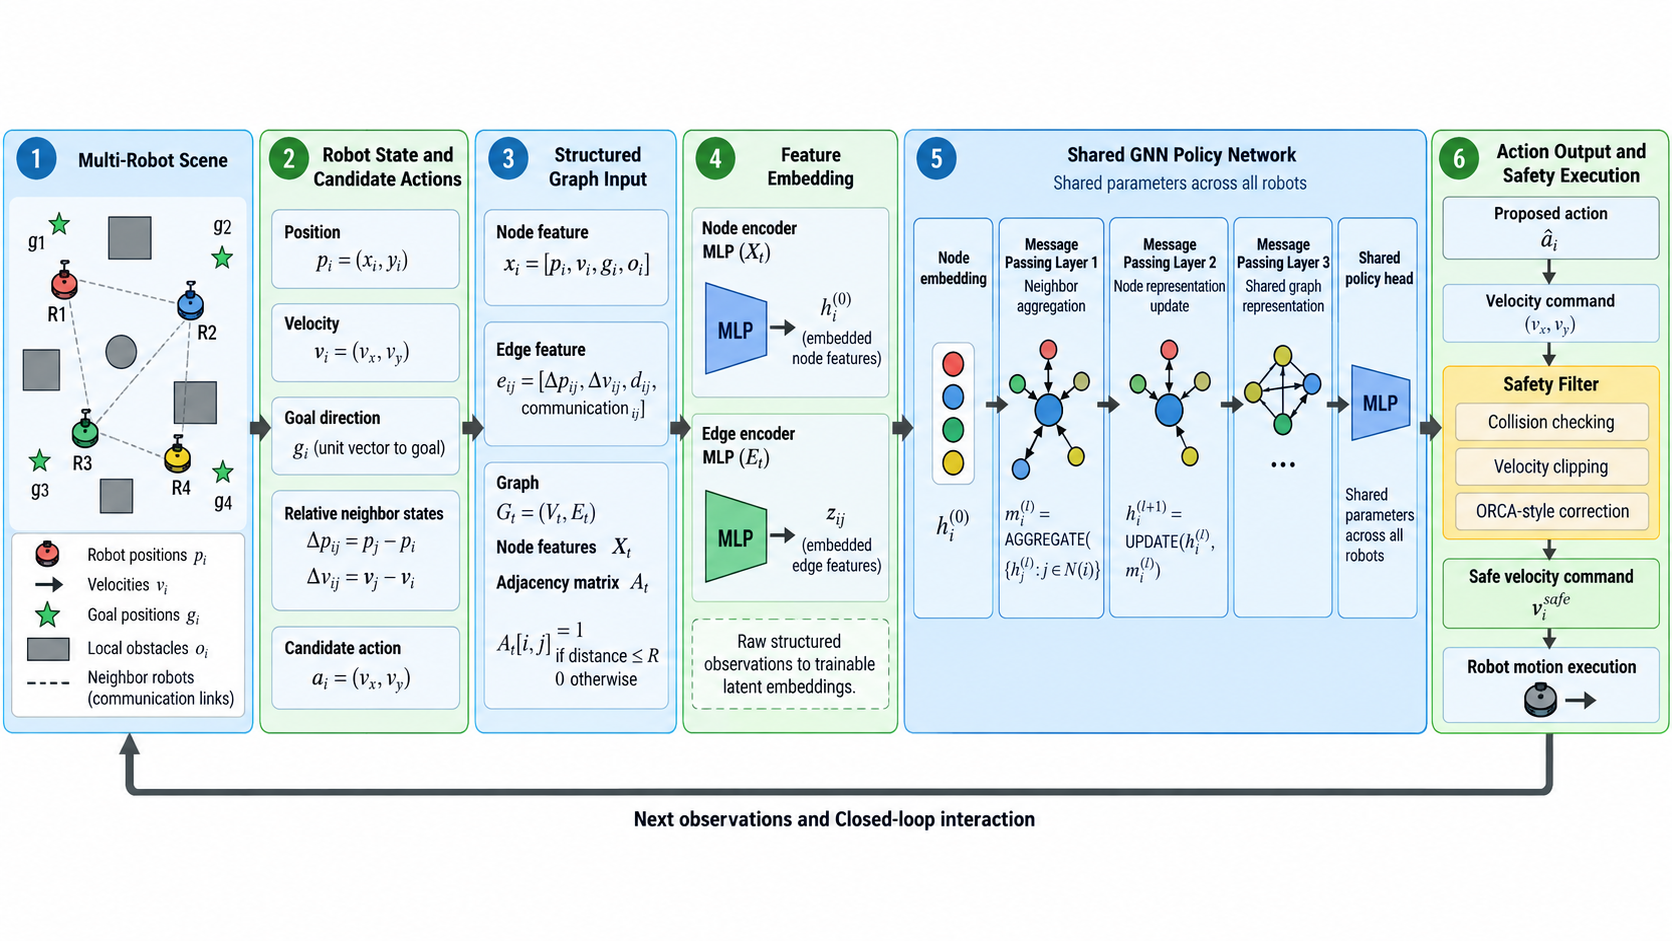
\includegraphics[width=\textwidth,trim=0 65bp 0 85bp,clip]{gnn_architecture_ai_fig1_draft_v2.png}
\caption{多机器人导航流程：机器人场景与状态、结构化图输入、特征嵌入、共享 GNN 推理，以及动作输出与可选安全过滤。执行后的运动反馈形成观测--动作闭环。}
\label{fig:arch}
\end{figure*}

\subsection{基线方法}
基线包括 A* 栅格跟踪、ORCA-style 局部排斥控制器，以及在有限方向与速度格点上采样的 RVO-style 控制器。RVO-style 根据预测邻居间距、障碍物占用和目标进度对候选速度评分。该控制器为本实验自行实现，并非经过形式验证的 RVO 参考实现。独立 MLP 在机器人间共享参数，但仅使用节点特征，不接收邻接矩阵。

\subsection{消息传递策略}
首先用线性层将节点特征映射为隐表示。每一层对邻居表示取平均，并将自身状态与变换后的邻域消息拼接后更新节点：
\begin{equation}
m_i^{(l)}=\tfrac{1}{\max(1,d_i)}{\textstyle\sum_j}A_{ij}h_j^{(l)},\;
h_i^{(l+1)}=\sigma(W_l[h_i^{(l)}\Vert\phi_l(m_i^{(l)})]).
\end{equation}
加入边特征后，消息形式为
\begin{equation}
m_i^{(l)}=\tfrac{1}{\max(1,d_i)}{\textstyle\sum_j}A_{ij}(\phi_l(h_j^{(l)})+\psi_l(e_{ij})),
\end{equation}
随后
$h_i^{(l+1)}=\mathrm{ReLU}(W_l[h_i^{(l)}\Vert m_i^{(l)}])$。本文使用 3 层消息传递、128 个隐藏单元与共享动作头，动作由 $\hat{u}_i=v_{\max}\tanh(f_\theta(h_i))$ 约束在可执行范围内。

\subsection{注意力变体}
两种注意力模型采用相同的输入、输出、数据与测试场景。邻域注意力 GNN 用查询、键、值上的多头注意力替换均值聚合，并由局部邻接矩阵掩蔽。Graph Transformer 使用动态邻接矩阵掩蔽的多头自注意力、残差连接与前馈块。两者均使用 128 个隐藏单元、4 个注意力头和共享策略头。

\subsection{训练目标}
单纯的动作模仿能够复现专家的局部行为，却无法保证闭环安全，因此本文以四项损失加权和进行训练：
\begin{equation}
\mathcal{L}=\lambda_a\mathcal{L}_{act}+\lambda_c\mathcal{L}_{col}
+\lambda_p\mathcal{L}_{prog}+\lambda_s\mathcal{L}_{smooth},
\end{equation}
其中 $\mathcal{L}_{act}=\frac{1}{|\mathcal{V}|}\sum_i\mathrm{Huber}(u_i,u_i^*)$ 为模仿项。记一步预测后的机器人对距离为 $d_{ij}'=\|p_i+\Delta t\,u_i-p_j-\Delta t\,u_j\|$，则 $\mathcal{L}_{col}=\frac{1}{N(N-1)}\sum_{i\neq j}[d_s-d_{ij}']_+^2$ 惩罚低于安全阈值的预测间距。其余两项为
\begin{equation}
\begin{aligned}
\mathcal{L}_{prog}&=\tfrac{1}{N}{\textstyle\sum_i}[\|g_i-p_i'\|-\|g_i-p_i\|]_+,\\
\mathcal{L}_{smooth}&=\tfrac{1}{N}{\textstyle\sum_i}\|u_i^t-u_i^{t-1}\|_2^2,
\end{aligned}
\end{equation}
其中 $[x]_+=\max(x,0)$。填充节点由 $q_i\in\{0,1\}$ 掩蔽，故每个节点损失写作 $\sum_i q_i\ell_i/\max(1,\sum_i q_i)$，补齐到 40 个节点的图仅在真实的机器人上训练。

多规模训练从四类地图中采样 5--40 个机器人的数据集，并将每张图补齐到 40 个节点。目标进度项惩罚偏离目标的运动，平滑项限制相邻时间步的动作变化。

\subsection{安全过滤器}
策略输出动作后，过滤器检查每一对近距离机器人，在速度裁剪之前施加对称修正。令 $\delta_{ij}=p_i-p_j$，$n_{ij}=\delta_{ij}/(\|\delta_{ij}\|+\epsilon)$。若 $\|\delta_{ij}\|<d_s+\tau$ 且 $(u_i-u_j)\cdot n_{ij}<0$，则
\begin{equation}
\begin{aligned}
\tilde{u}_i&=u_i+\tfrac{\kappa_{ij}}{2}n_{ij},\quad
\tilde{u}_j=u_j-\tfrac{\kappa_{ij}}{2}n_{ij},\\
\kappa_{ij}&=-(u_i-u_j)\cdot n_{ij}+[d_s+\tau-\|\delta_{ij}\|]_+,
\end{aligned}
\end{equation}
之后将每个 $\tilde{u}_i$ 裁剪至 $v_{\max}$。过滤器仅在推理阶段启用，其效果在第~\ref{sec:results}~节中单独评估。

\section{实验设计}

实验覆盖四类地图——\textit{crossing}、\textit{open}、\textit{random} 与 \textit{narrow}——以及 5、10、20、30、40 个机器人。开发数据使用固定种子，每类 20 个回合、每回合至多 160 个时间步。主实验覆盖 $4\times3\times5\times10=600$ 个回合，包含三种机器人规模、五种方法与十个固定测试种子；扩展学习模型对比包含四种学习策略的 480 个回合；多规模测试包含 30 个未见种子（100--129）下的 1800 个安全过滤回合与 1800 个未过滤回合。所有方法共享初始状态、目标、障碍物、动作限制与终止规则。数据以压缩 NPZ 形式保存，包含特征、邻接、动作、位置、奖励、障碍物、地图、专家标识与步索引。

报告指标包括目标到达率、严格无物理碰撞成功率、安全距离违规事件、物理碰撞事件、最小机器人间距、路径长度、最终目标误差与每控制步平均计算时间。均值、标准差与 95\% 置信区间均由回合级结果计算；0.72~m 的违规与 0.56~m 的物理碰撞始终分列报告。训练使用单张 24~GB GPU，批大小为 128。

\section{实验结果}
\label{sec:results}

\subsection{主实验比较}
表~\ref{tab:main} 汇总了 600 个回合的主实验结果。A* 在各规模下的任务成功率均为 1.000。RVO-style 的成功率为 0.975--1.000，路径最短，平均控制时间从 5 个机器人时的 7.8~ms 增至 20 个机器人时的 87.4~ms，约为原来的 11 倍。ORCA-style 在各规模下的控制时间最低，最小机器人间距最大。本组学习策略中，独立 MLP 的成功率较高，为 0.725--0.875。

均值聚合 GNN 在 5、10、20 个机器人下的成功率分别为 0.625、0.725 和 0.700，低于 MLP，但各规模下的最小机器人间距均大于 MLP。该 GNN 检查点仅使用 10 个机器人的数据训练，因此 5 和 20 个机器人的结果反映跨规模泛化能力。后续图结构消融在同一网络上比较有边与无边配置，以区分消息传递的作用。

\begin{table*}[t]
\caption{主实验比较（四类地图 $\times$ 十个固定测试种子，每格 40 个回合）。Succ 为目标成功率；Coll 为碰撞事件数，计入距离低于 0.72~m 安全阈值的状态转入次数；Sep 为最小机器人间距（m）；$T$ 为每控制步平均计算时间（ms）。}
\label{tab:main}
\centering
\scriptsize
\setlength{\tabcolsep}{3pt}
\begin{tabular}{lcccccccccccc}
\toprule
& \multicolumn{4}{c}{5 个机器人} & \multicolumn{4}{c}{10 个机器人} & \multicolumn{4}{c}{20 个机器人}\\
\cmidrule(lr){2-5}\cmidrule(lr){6-9}\cmidrule(lr){10-13}
方法 & Succ & Coll & Sep & $T$ & Succ & Coll & Sep & $T$ & Succ & Coll & Sep & $T$\\
\midrule
A*         & 1.000 & 1.925  & 0.280 & 0.512 & 1.000 & 6.075  & 0.098 & 1.205 & 1.000 & 30.700 & 0.035 & 2.493\\
ORCA-style & 0.775 & 1.425  & 0.396 & 0.213 & 0.825 & 3.825  & 0.296 & 0.486 & 0.825 & 13.500 & 0.230 & 1.303\\
RVO-style  & 0.975 & 1.825  & 0.294 & 7.779 & 1.000 & 5.575  & 0.131 & 24.941 & 1.000 & 23.325 & 0.062 & 87.373\\
MLP        & 0.725 & 2.575  & 0.191 & 0.342 & 0.850 & 5.400  & 0.095 & 0.483 & 0.875 & 27.400 & 0.038 & 0.775\\
GNN        & 0.625 & 1.850  & 0.224 & 0.683 & 0.725 & 5.675  & 0.149 & 0.828 & 0.700 & 28.675 & 0.041 & 1.129\\
\bottomrule
\end{tabular}
\end{table*}

\begin{figure}[t]
\centering
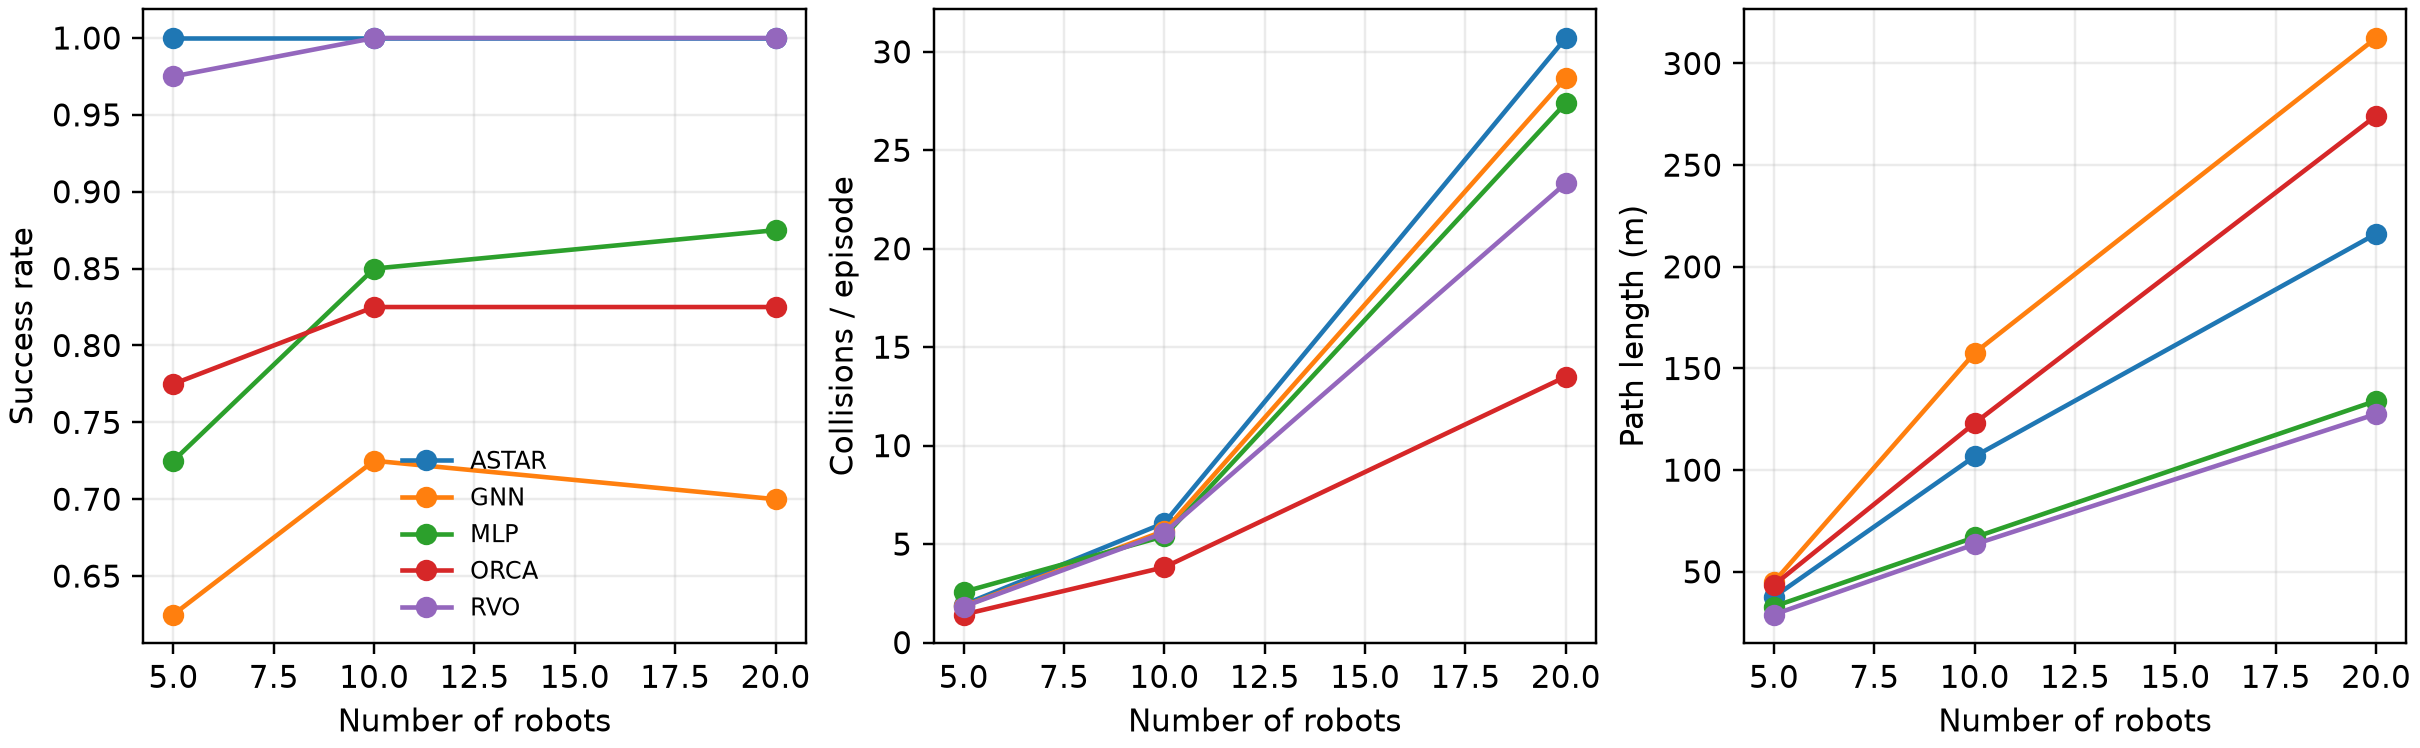
\includegraphics[width=\columnwidth]{baselines_final.png}
\caption{600 回合主实验中各方法在不同机器人规模下的目标到达率、路径长度与控制时间对比。}
\label{fig:baselines}
\end{figure}

\begin{figure*}[t]
\centering
\begin{minipage}[t]{0.49\textwidth}
\centering
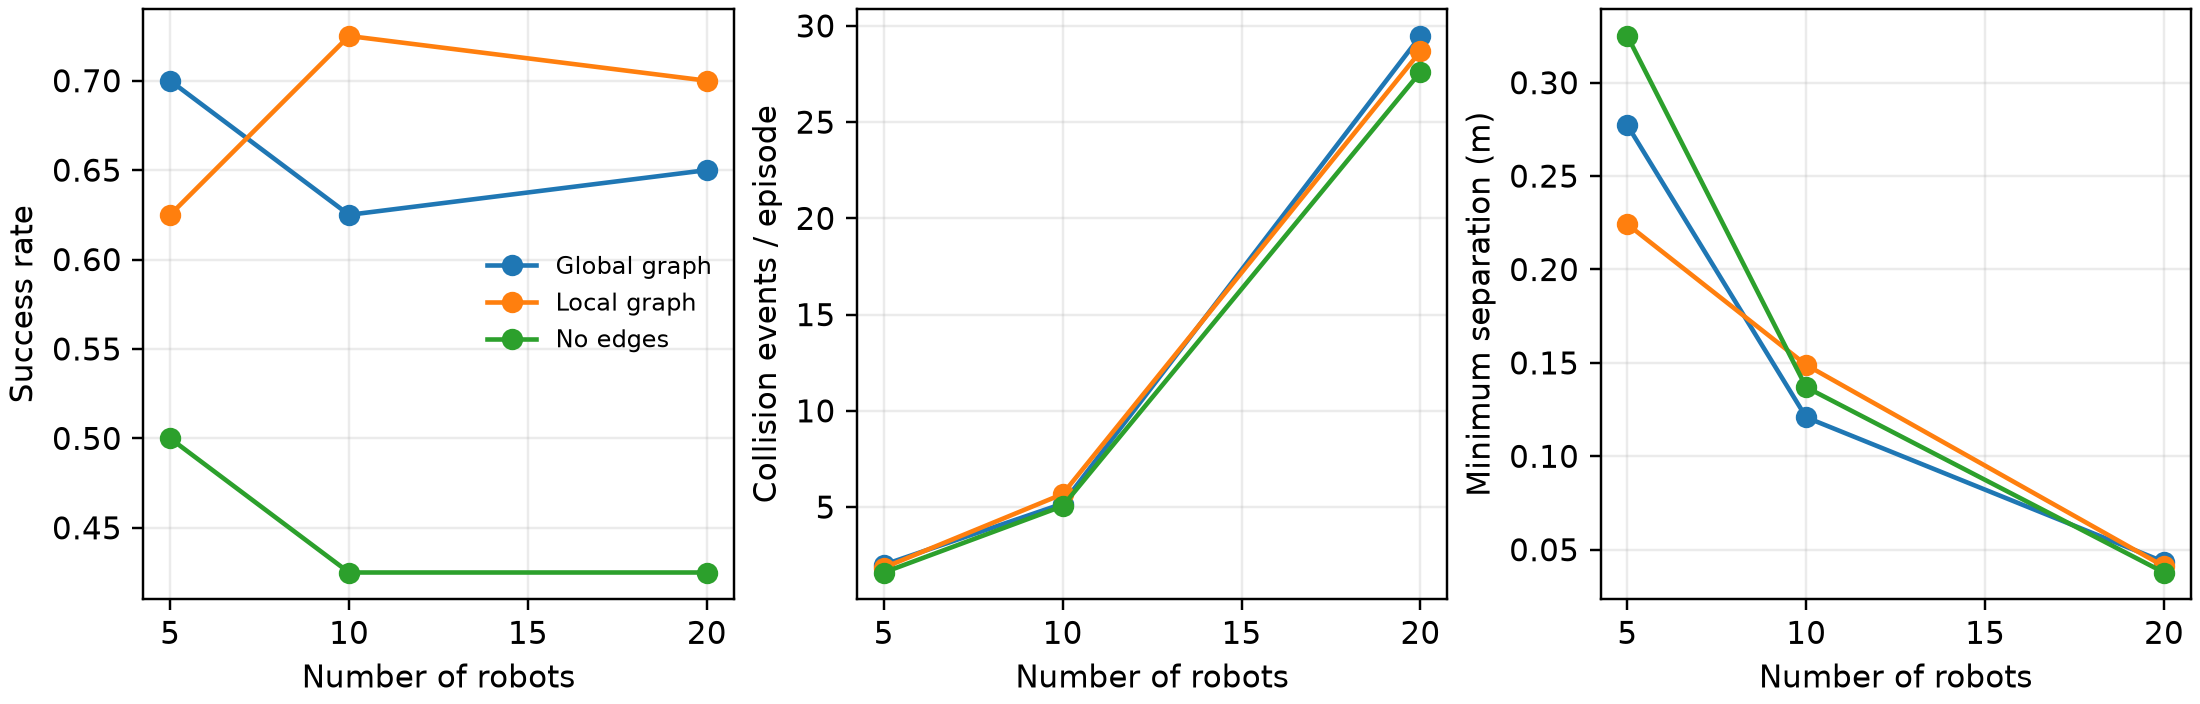
\includegraphics[width=\linewidth]{ablation_graph_final.png}\\
(a) 图结构
\end{minipage}\hfill
\begin{minipage}[t]{0.49\textwidth}
\centering
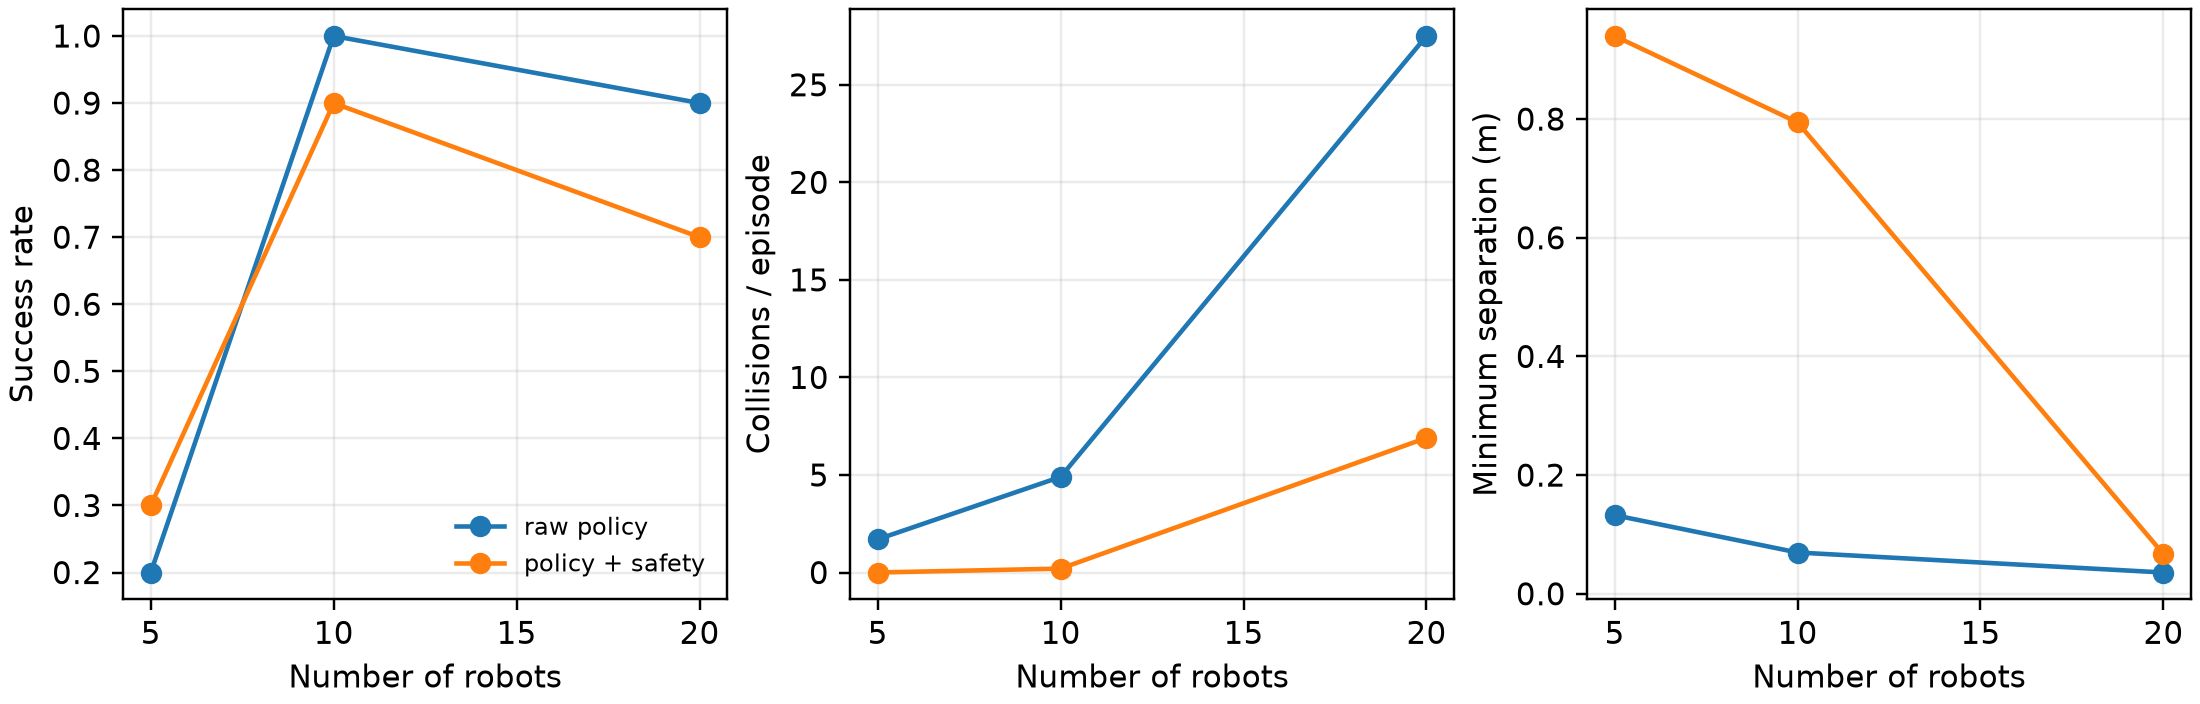
\includegraphics[width=\linewidth]{ablation_safety_final.png}\\
(b) 安全过滤器
\end{minipage}
\caption{5、10、20 个机器人下的消融结果。(a) 无边、局部图与全局图的目标到达率。(b) 安全过滤前后的目标到达率、安全距离违规事件与最小间距。}
\label{fig:ablations}
\end{figure*}

\begin{figure}[t]
\centering
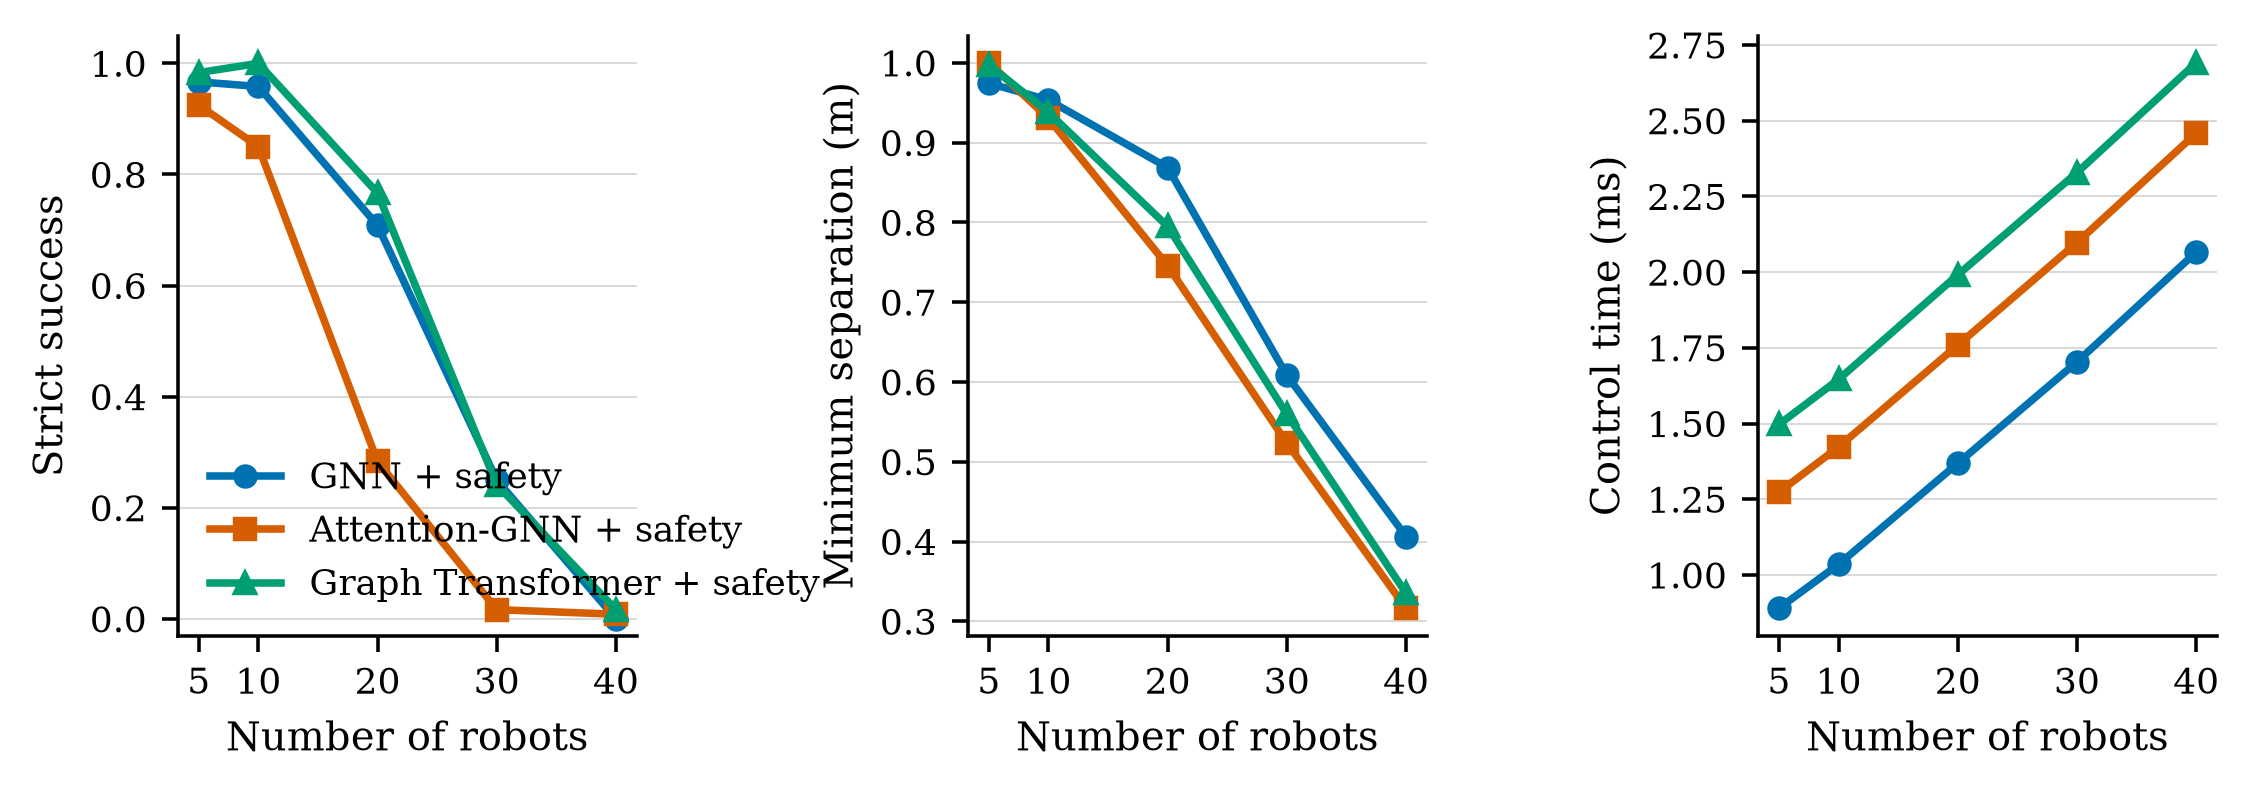
\includegraphics[width=\columnwidth]{multiscale_safety_scaling.png}
\caption{安全过滤下不同机器人规模的严格无碰撞成功率、最小间距与平均控制时间。机器人数量超过 20 后，无碰撞成功率下降。}
\label{fig:scaling}
\end{figure}

\begin{figure*}[!t]
\centering
\begin{minipage}[t]{0.30\textwidth}
\centering
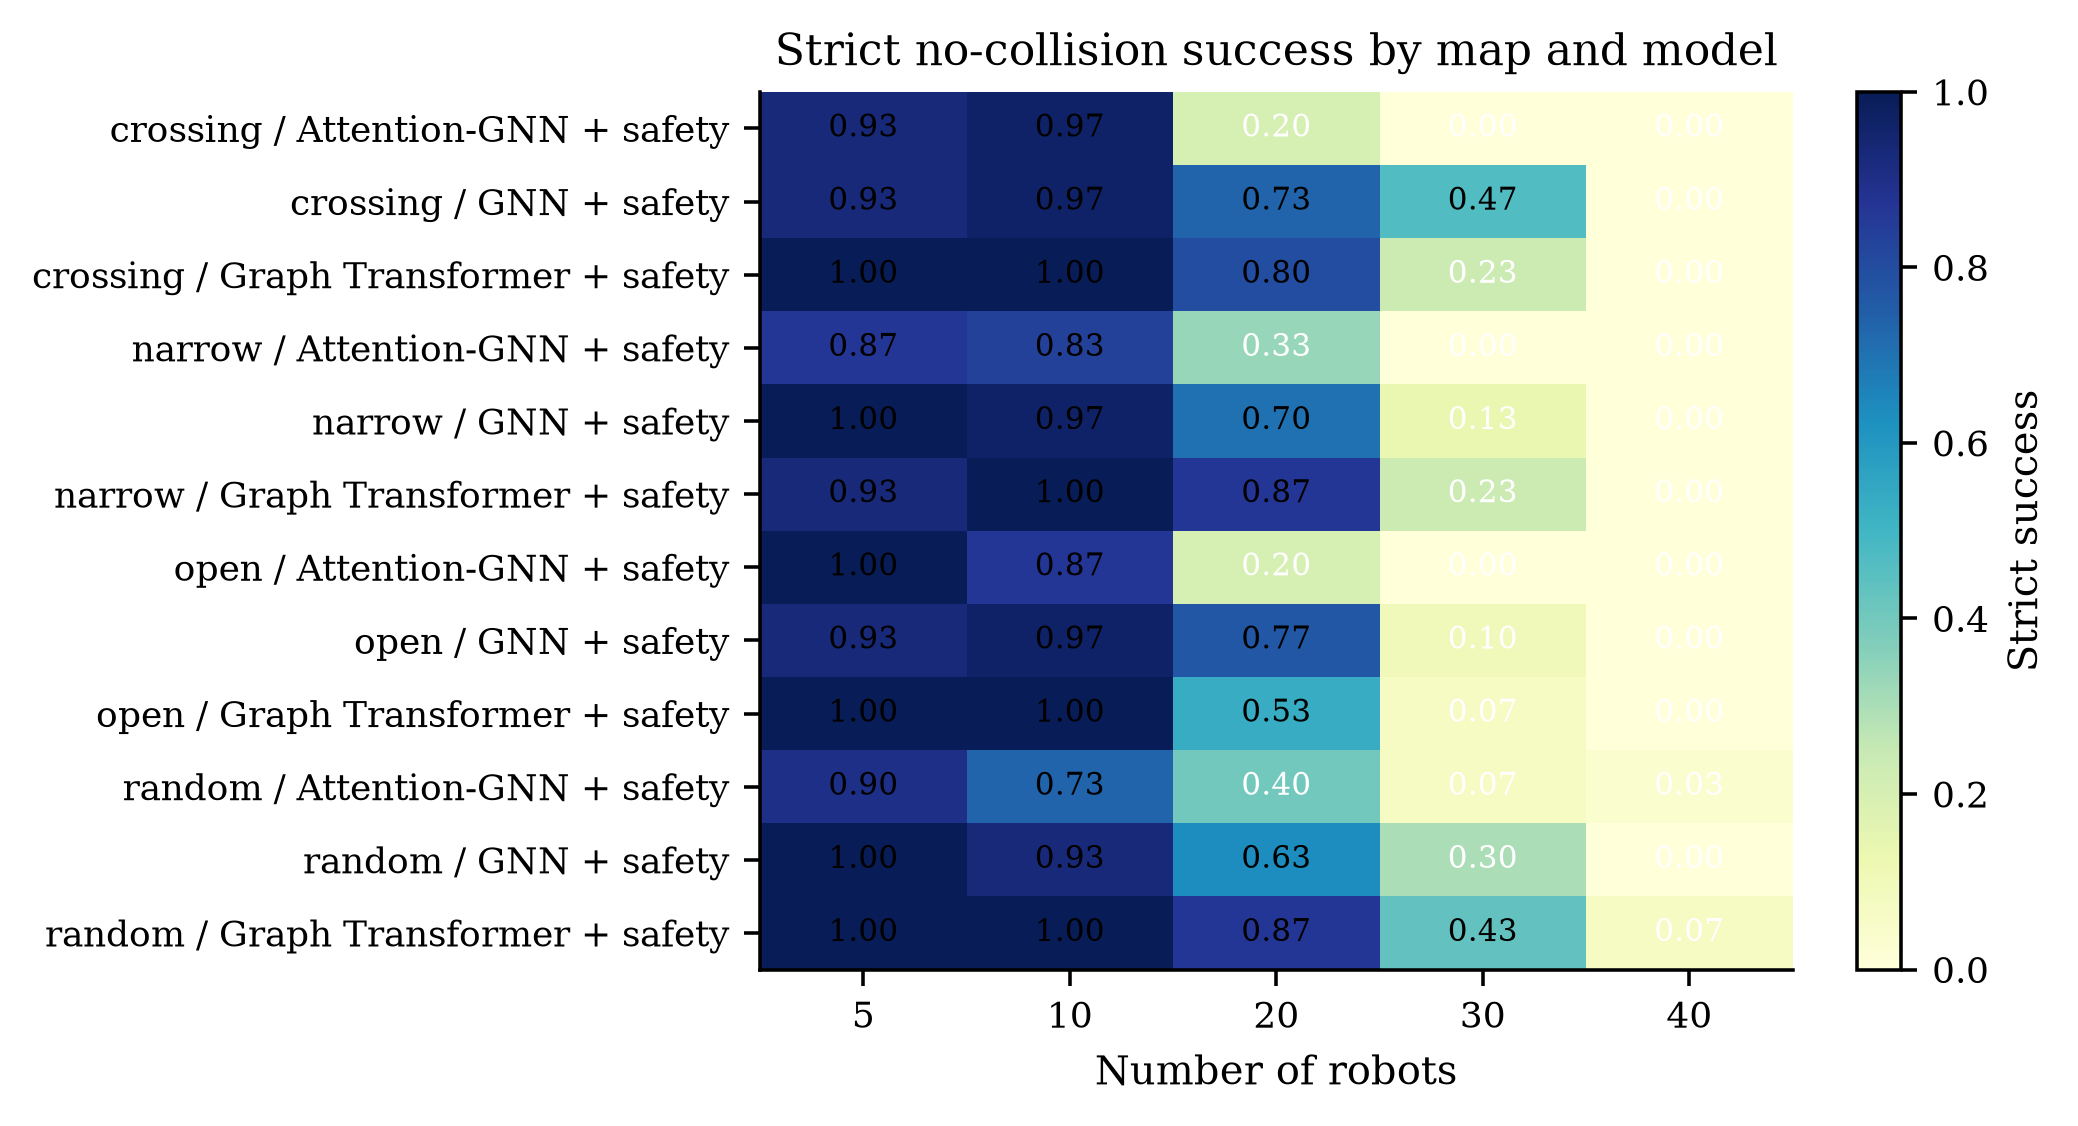
\includegraphics[width=\linewidth]{multiscale_map_heatmap.png}\\
(a) 分地图与密度的严格成功率
\end{minipage}\hfill
\begin{minipage}[t]{0.68\textwidth}
\centering
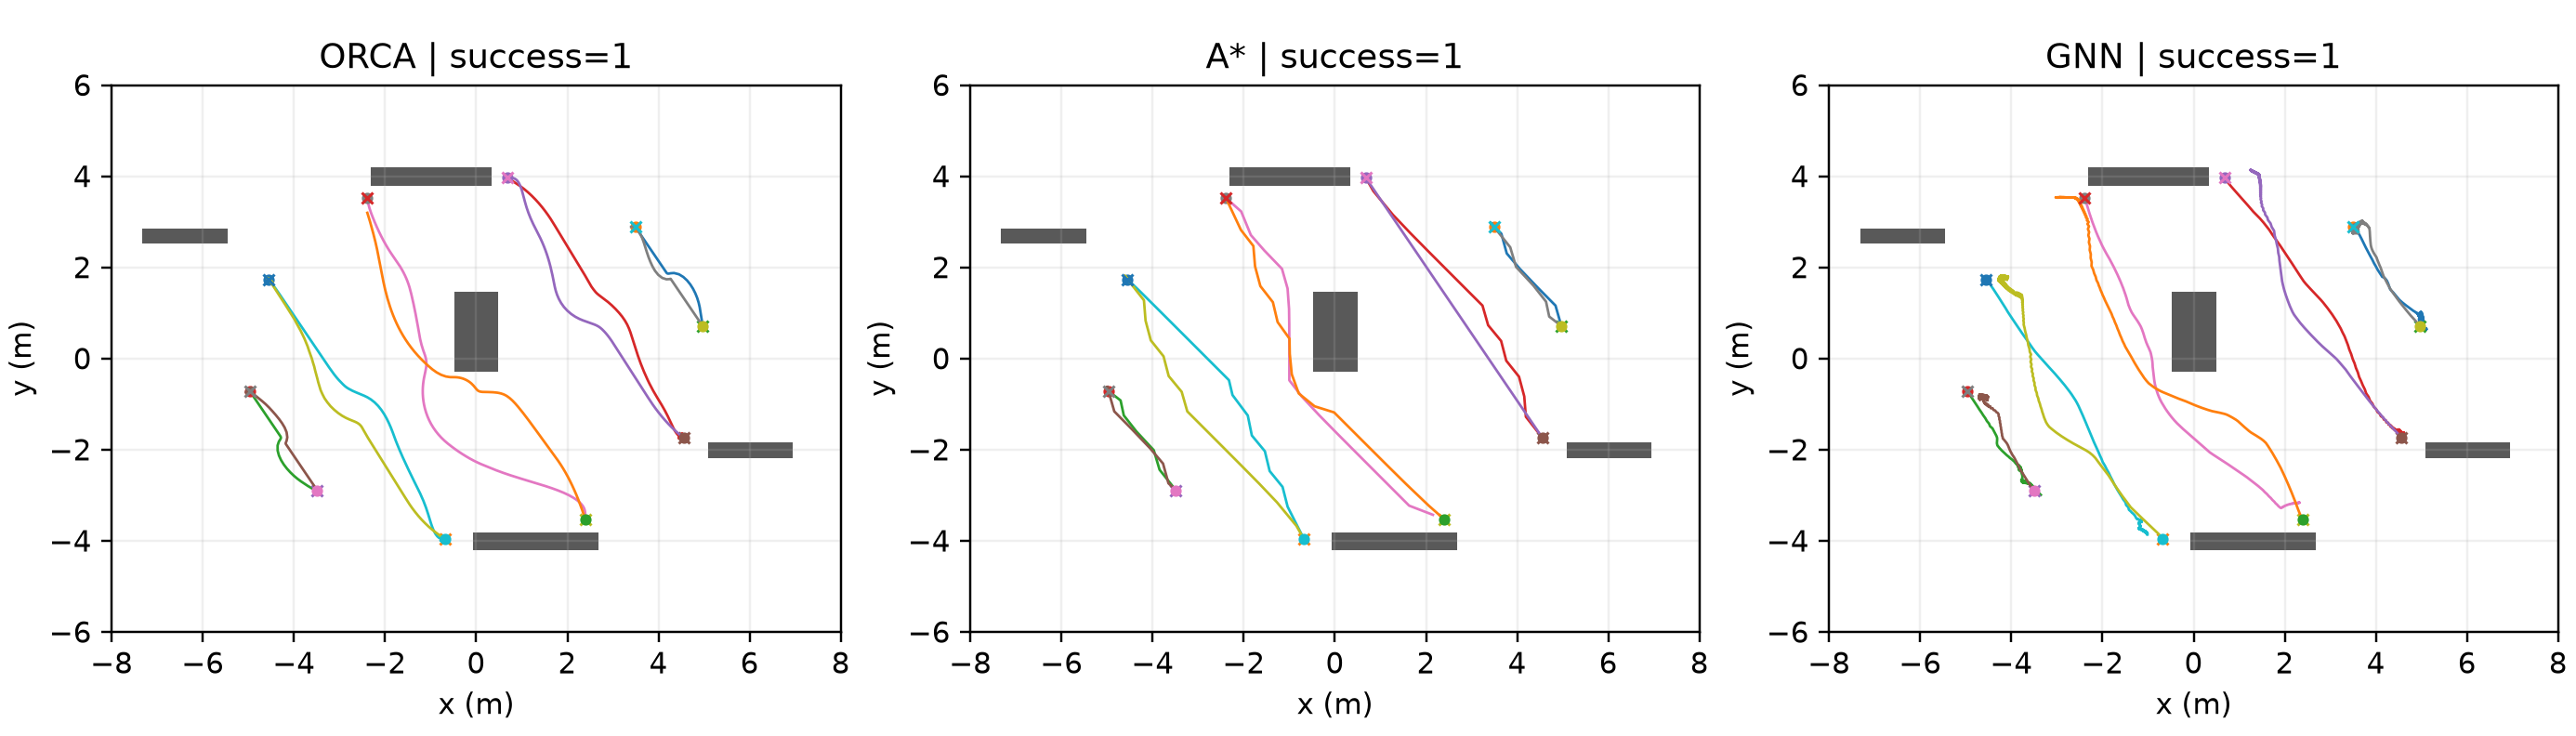
\includegraphics[width=\linewidth]{trajectories_final.png}\\
(b) 典型轨迹
\end{minipage}
\caption{(a) 各地图族与不同群体规模下的严格无碰撞成功率；\textit{random} 与 \textit{narrow} 布局在高密度下最具挑战性。(b) 典型轨迹，通信边以瞬时连线的形式绘制于半径内的机器人之间。}
\label{fig:mapstraj}
\end{figure*}

\subsection{注意力与 Transformer 变体}
表~\ref{tab:learned} 比较了四种学习策略在 480 个回合上的表现。MLP、GNN、Graph Transformer 和邻域注意力 GNN 的目标到达率分别为 0.817、0.683、0.558 和 0.342，严格无碰撞成功率分别为 0.017、0.008、0.058 和 0.025。Graph Transformer 的严格成功率最高，平均控制时间为 1.365~ms，GNN 则为 0.856~ms。邻域注意力将平均最小间距提高至 0.259~m，但目标到达率降低，单步耗时为 1.298~ms。上述未经过滤的策略仍不足以实现可靠的无碰撞导航。

\begin{table}[t]
\caption{学习策略对比（480 个回合）。严格率要求到达目标且任意机器人对的距离从未低于 0.56~m 的物理直径阈值；碰撞事件为物理碰撞事件数。}
\label{tab:learned}
\centering
\footnotesize
\setlength{\tabcolsep}{3pt}
\begin{tabular}{lrrrrr}
\toprule
模型 & 成功率 & 严格率 & 碰撞事件 & 最小间距/m & 时间/ms\\
\midrule
MLP        & 0.817 & 0.017 & 9.250 & 0.108 & 0.515 \\
GNN        & 0.683 & 0.008 & 8.825 & 0.138 & 0.856 \\
邻域注意力 & 0.342 & 0.025 & 8.167 & 0.259 & 1.298 \\
Transformer & 0.558 & 0.058 & 8.833 & 0.221 & 1.365 \\
\bottomrule
\end{tabular}
\end{table}

\subsection{图结构消融}
图结构消融比较局部图、全局图与无边配置（图~\ref{fig:ablations}a）。10 个机器人时，局部图成功率为 0.725，同等容量的无边策略为 0.425，提高了 30 个百分点；5 和 20 个机器人时分别提高 12.5 和 27.5 个百分点。全连接未进一步改善局部通信的效果：10 个机器人时，全局图与局部图成功率分别为 0.625 和 0.725。结果表明，局部邻居信息交换有助于目标到达，但两种图策略仍存在碰撞。

\subsection{安全层消融}
安全过滤消融在 60 个回合上比较原始 GNN 动作与修正后的动作（图~\ref{fig:ablations}b）。10 个机器人时，平均安全距离违规事件由 4.900 降至 0.200，平均最小间距由 0.069~m 增至 0.794~m，目标到达率由 1.000 降至 0.900。20 个机器人时，违规事件由 27.500 降至 6.900，目标到达率由 0.900 降至 0.700，平均最小间距为 0.067~m。动作修正改善了间距，但也可能阻碍目标趋近；其在 20 个机器人下的效果有限，仍需研究训练阶段的安全约束。

\subsection{通信半径}
扩大通信半径会增加每个机器人的图邻居。10 个机器人时，2.0~m 半径对应平均度 0.463、成功率 0.200；3.4~m 和 5.5~m 半径对应平均度 2.283 和 4.420，成功率均为 1.000；全局图平均度为 9.000，成功率为 0.900。5 个机器人时，成功率由 2.0~m 半径下的 0.100 增至全局图下的 1.000。结果表明，过小半径可能限制信息交换，而局部通信范围足够后，继续增加邻居未必提高成功率。各测试配置下的控制时间约为 0.8--1.5~ms，全局连通仍未消除物理碰撞。

\subsection{多规模压力测试}
表~\ref{tab:multiscale} 汇总了每种配置采用 30 个未见种子的 1800 回合安全过滤测试。5 和 10 个机器人时，GNN 严格无碰撞成功率分别为 0.967 和 0.958，测试中未记录到物理碰撞；同条件下 Graph Transformer 分别为 0.983 和 1.000。20 个机器人时，GNN 与 Transformer 的目标到达率分别为 0.758 和 0.842，严格成功率分别为 0.708 和 0.767。30 和 40 个机器人时，GNN 严格成功率降至 0.250 和 0.000，Transformer 降至 0.242 和 0.017。40 个机器人时，两者每回合平均物理碰撞事件分别为 6.883 和 9.025，最小间距约为 0.4~m。GNN 平均控制时间从 5 个机器人时的 0.890~ms 增至 40 个机器人时的 2.066~ms。

未加过滤时，GNN 在各规模下的目标到达率为 0.975--1.000，但严格无碰撞成功率在 5 个机器人时为 0.092，更大规模时均为 0.000；未过滤 Transformer 的严格成功率不超过 0.117。安全过滤提高了无碰撞到达率，在 5--10 个机器人下尤为明显，同时降低了目标到达率。30--40 个机器人时，过滤后策略的完成率和安全性均下降，限制了其在这些密度下的应用。

\begin{table}[t]
\caption{安全过滤下的多规模测试（30 个未见种子，1800 个回合，四类地图聚合，按机器人数量索引）。严格成功率要求到达目标且不发生物理碰撞。}
\label{tab:multiscale}
\centering
\footnotesize
\setlength{\tabcolsep}{4pt}
\resizebox{\columnwidth}{!}{%
\begin{tabular}{lccccc}
\toprule
模型 & 5 & 10 & 20 & 30 & 40\\
\midrule
\multicolumn{6}{l}{\textit{目标到达率 / 严格无碰撞成功率}}\\
GNN               & 0.967/0.967 & 0.958/0.958 & 0.758/0.708 & 0.400/0.250 & 0.042/0.000\\
Graph Transformer & 0.983/0.983 & 1.000/1.000 & 0.842/0.767 & 0.467/0.242 & 0.108/0.017\\
\addlinespace
\multicolumn{6}{l}{\textit{每回合物理碰撞事件数}}\\
GNN               & 0.000 & 0.000 & 0.075 & 1.158 & 6.883\\
Graph Transformer & 0.000 & 0.000 & 0.217 & 2.267 & 9.025\\
\addlinespace
\multicolumn{6}{l}{\textit{最小间距（m）/ 控制时间（ms）}}\\
GNN               & 0.97/0.89 & 0.95/1.04 & 0.87/1.37 & 0.61/1.70 & 0.41/2.07\\
Graph Transformer & 1.00/1.50 & 0.94/1.65 & 0.80/1.99 & 0.56/2.33 & 0.34/2.69\\
\bottomrule
\end{tabular}}
\end{table}

\subsection{训练种子稳定性}
三个独立训练的 GNN 检查点在 5、10、20 个机器人下的平均成功率分别为 $0.517\pm0.388$、$0.767\pm0.161$ 和 $0.850\pm0.115$。标准差由各检查点的平均成功率计算。5 个机器人下的差异最大，表明该场景对训练种子较为敏感。本项分析单独考察训练差异，前述对比则报告固定检查点在各测试回合上的平均表现。

\section{局限性与结论}

本文提出了结合相对运动边特征、联合模仿训练目标和外部安全过滤器的多机器人动态图策略。局部消息传递提高了相对同等容量无边策略的目标到达率，全局连通则未带来一致的额外收益。安全过滤增大了机器人间距，并在多规模测试的 5--10 个机器人场景中实现了较高的无碰撞成功率。GNN 在各测试规模下保持毫秒级控制时间。

实验也表明，主对比中均值聚合 GNN 的目标到达率低于独立 MLP，30--40 个机器人下的严格无碰撞成功率明显下降。主实验 GNN 仅在单一规模上训练，规则专家也限制了可供模仿的行为。RVO-style 基线采用有限候选采样，并非经过验证的 RVO 实现；当前验证仍限于仿真。后续将研究显式安全约束训练、与 RVO 参考实现的对比、跨地图泛化及真实机器人实验。

\bibliographystyle{IEEEtran}
% IEEEtran 参考文献默认 \footnotesize；略微收紧以在六页限制内保留全部引用。
\renewcommand{\footnotesize}{\fontsize{7.5}{8.6}\selectfont}
\bibliography{references}

\end{document}
